% unofficial poster template for Trinity College Dublin
% which is a fork of the unofficial University of Texas at Arlington Math Poster template:
% which is a fork of the unofficial University of Lethbridge Poster template: https://www.overleaf.com/latex/templates/university-of-lethbridge-unofficial-poster-template/nddfzgvqvfwf
% which is a fork of unofficial University of Alberta Poster template: 
% which is a fork of Yale template: https://www.overleaf.com/latex/templates/yale-poster-template/rjpgqfgvsjcv
% which is a fork of the UMich template https://www.overleaf.com/latex/templates/university-of-michigan-umich-poster-template/xpnqzzxwbjzc
% which is fork of the MSU template https://www.overleaf.com/latex/templates/an-unofficial-poster-template-for-michigan-state-university/wnymbgpxnnwd
% which is a fork of https://www.overleaf.com/latex/templates/an-unofficial-poster-template-for-new-york-university/krgqtqmzdqhg
% which is a fork of https://github.com/anishathalye/gemini
% also refer to https://github.com/k4rtik/uchicago-poster


\documentclass[final]{beamer}

% ====================
% Packages
% ====================

\usepackage[T1]{fontenc}
\usepackage[utf8]{luainputenc}
\usepackage{lmodern}
\usepackage[size=custom, width=122,height=91, scale=1.2]{beamerposter}
\usetheme{gemini}
\usecolortheme{msu}
\usepackage{graphicx}
\usepackage{booktabs}
\usepackage{tikz}
\usepackage{pgfplots}
\pgfplotsset{compat=1.14}
\usepackage{anyfontsize}

% ====================
% Lengths
% ====================

% If you have N columns, choose \sepwidth and \colwidth such that
% (N+1)*\sepwidth + N*\colwidth = \paperwidth
\newlength{\sepwidth}
\newlength{\colwidth}
\setlength{\sepwidth}{0.025\paperwidth}
\setlength{\colwidth}{0.3\paperwidth}

\newcommand{\separatorcolumn}{\begin{column}{\sepwidth}\end{column}}

% ====================
% Title
% ====================

\title{Fibonacci numbers in Ford Circles and Golden Ratio}

\author{Woojin Juhn, Jingyuan Zhang}
% add following line if you have co-author(s)
% Coauthor One$^{2}$, Coauthor Two$^{3}$

\institute[shortinst]{\textbf{M 325K}, Discrete Mathematics}

% ====================
% Footer (optional)
% ====================

\footercontent{Mathposium \hfill
  \href{mailto:youremail@tcd.ie}{woojinjuhn@utexas.edu}}
% (can be left out to remove footer)

% ====================
% Logo
% ====================

% use this to include logos on the left and/or right side of the header:
% Left: institution
 \logoleft{
\includegraphics[height=6cm]{logos/DofM.png}}
 \logoright{
\includegraphics[height=6cm]{logos/cns_logo.png}}
% Right: funding agencies and other affilations 
%\logoright{\includegraphics[height=7cm]{logos/NSF.eps}}

% ====================
% Body
% ====================

\begin{document}



\begin{frame}[t]
\begin{columns}[t]
\separatorcolumn

\begin{column}{\colwidth}

  \begin{block}{Abstract}

Fibonacci numbers appear unexpectedly often in mathematics. We will explore how Fibonacci numbers serve as a coordinate that represents the trace of a Ford circle as we extend them into 2-dimensional points. Also, we aim to show how the “Golden Ratio” is derived from using the ratios of Fibonacci numbers.  Finally, we will combine the concepts of the Ford Circle and the Golden Ratio and show that the 2-dimensional points are on the same circle with the radius of the Golden Ratio.
 \end{block}

  \begin{block}{Background and Basic Properties of the Fibonacci Numbers}

   

   In mathematics, the term Fibonacci sequence is the series of numbers where each number is the sum of the two preceding numbers. 0, 1, 1, 2, 3, 5, 8, 13, 21, 34, 55, … is a Fibonacci sequence, for example, and the numbers that are part of this sequence are known as the Fibonacci numbers. 
The pattern of this Fibonacci sequence is given by $F_{0}=0,\quad F_{1}=1$ and the recursive formula $F_{n}=F_{n-1}+F_{n-2}  , \quad n>2$.
For Fibonacci sequence, the ratio of consecutive terms is approaching a constant number $\frac{\sqrt{5}}{2}$ . We called this number the golden ratio and it appears in many fields of math.
There are some basic identities of involving Fibonacci sequence, and we will prove by mathematical induction. 

\textbf{Lemma 1.}	$F_{n+m} = F_{n-1} \cdot F_m + F_n \cdot F_{m+1}

For $m = 1$,
\newline $F_{n+1} = F_{n-1} \cdot F_1 + F_n \cdot F_2$, \quad $F_{1} = 1 , \quad F_{2} =1$
\newline $F_{n+1} = F_n + F_{n-1} = F_{n-1} \cdot F_1 + F_n \cdot F_2$
\newline \therefore \quad$F_{n+1} = F_{n-1} \cdot F_1 + F_n \cdot F_2$

For $m = 2$,
\newline $F_{n+2} = F_{n-1} \cdot F_2 + F_n \cdot F_3$, \quad $F_{2} = 1 , \quad F_{3} = 2$
\newline $F_{n+2} = F_{n+1} + F_n = F_{n-1} + F_n + F_n = F_{n-1} + 2F_n$
\newline \therefore \quad$F_{n+2} = F_{n-1} \cdot F_2 + F_n \cdot F_3$

Suppose the formula to be true for $m = k$ and for $m = k + 1$. 

\newline For $m = k + 2$,
\newline $F_{n+k} = F_{n-1} \cdot F_k + F_n \cdot F_{k+1}$
\newline $F_{n+k+1} = F_{n-1} \cdot F_{k+1} + F_n \cdot F_{k+2}$
\newline If we add these two equations term by term, 
\newline $F_{n+k} + F_{n+k+1} = F_{n-1} \cdot F_k + F_n \cdot F_{k+1} + F_{n-1} \cdot F_{k+1} + F_n \cdot F_{k+2}$
\newline $F_{n+k+2} = F_{n-1} \cdot F_{k+2} + F_n \cdot F_{k+3}$

\newline Therefore, the initial formula holds true for all values of $m$.


\textbf{Lemma 2.}    $F_n^2 - F_{n-1}F_{n+1} = (-1)^{n+1}$

For $n = 2$, \quad\quad\quad\quad\quad\quad\quad\quad\quad For $n = 3$,
\newline $F_2^2 - F_1 \cdot F_3 = (-1)^3$ \quad\quad\quad\quad\quad $F_3^2 - F_2 \cdot F_4 = (-1)^4$ 
\newline $F_{1} = 1 , F_{2} = 1 , F_{3} = 2$ \quad\quad\quad\quad $F_{2} = 1 , F_{3} = 2 , F_{4} = 3$
\newline $F_2^2 - F_1 \cdot F_3 = 1 - 2 = -1$ \quad\quad $F_3^2 - F_2 \cdot F_4 = 4 - 3 = 1$
\newline \therefore \quad$F_2^2 - F_1 \cdot F_3 = (-1)^3$ \quad\quad\quad \therefore \quad$F_3^2 - F_2 \cdot F_4 = (-1)^4$

Suppose the formula to be true for $m = k$. 

\newline For $m = k + 1$,
\newline $F_{n+1}^2 - F_nF_{n+2} = F_{n+1}^2 - F_n(F_n + F_{n+1})$
\newline =$F_{n+1}(F_{n+1} - F_n) - F_n^2$
\newline =$F_{n+1}F_{n-1} - F_n^2$
\newline =$-(-1)^{n+1}$
\newline =$(−1)^{n+2}$

\newline Therefore, the initial formula holds true for all values of $n.

  \end{block}


\end{column}

\separatorcolumn

\begin{column}{\colwidth}

  \begin{block}{Extension}

    Although the Fibonacci sequence seem to be a one dimensional object, we can extend it to two dimension by creating series of tuples relating to Fibonacci sequence.
    Here is how we construct the two-dimensional points:
    $\left( \frac{F_{2n}}{F_{2n+1}}, \: \frac{1}{F_{2n}} \right)$
    \newline
    Below is what the series of points looks like on the x-y plane.
    \begin{figure}
        \centering
        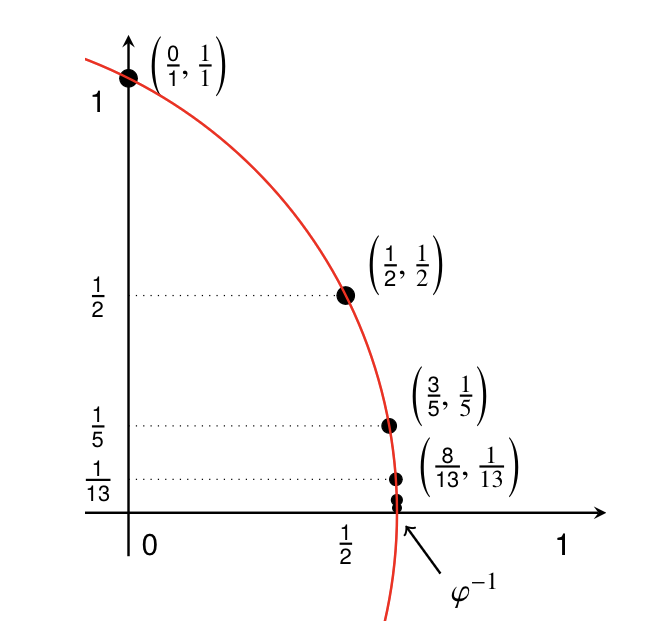
\includegraphics[width=0.5\linewidth]{截屏2024-03-30 下午4.01.58.png}
        \caption{Series of tuples[1]}
        \label{fig:enter-label}
    \end{figure}
    From this figure, we may guess that these points are concyclic(on the same circle), and this is in fact true!
    All the points are on the same circle centered at $\left(-\frac{1}{2}, \: 0 \right)$ of radius $\frac{\sqrt{5}}{2}$.
    
    \newline
    \textbf{Proof.}
    
    \newline
    To prove that  the the points are concyclic is the same as proving the folowing quadratic circle equation. (Denote $m = 2n$)
    \newline
    $(\frac{F_{m}}{F_{m+1}} \: + \frac{1}{2})^{2} \: + (\frac{1}{F_{m+1}})^2 = \frac{5}{4}$
    
    \newline
    Since the equation is saying that all points in this series have a constant distance $\frac{\sqrt{5}}{2}$ from the point $\left(-\frac{1}{2}, \: 0 \right)$
    \newline
    After squaring we get: $\frac{F_{m}^2}{F_{m+1}^2} \; + \frac{1}{4} \; + \frac{F_{m}}{F_{m+1}} + \frac{1}{F_{m+1}^2} = \frac{5}{4}$
    \newline
    We first collect like terms: $\frac{1+F_{m}^2}{F_{m+1}} + \frac{F_{m}}{F_{m+1}} = 1$
    \newline
    We then multiply both side by $F_{m+1}^2$: $1\;+F_{m}^2 + F_{m}F_{m+1} = F_{m+1}^2$
    \newline
    After rearranging we get: $F_{m}^2+1 = F_{m+1}^2 - F_{m}F_{m+1}$
    \newline
    From Lemma 2: $F_{m}^2+1 = F_{m+1}F_{m-1}$, the equation turns into $F_{m+1}F_{m-1} = F_{m+1}^2 - F_{m}F_{m+1}$.
    \newline
    After rearranging the right hand side of the equation:
    $F_{m+1}F_{m-1} = F_{m+1}(F_{m+1} - F_{m})$
    Then we use the definition of the Fibonacci sequence, and we get a identity equation:
    $F_{m+1}F_{m-1} = F_{m+1}F_{m-1}$.
    Hence, we are convinced that this equation always holds.
    
    \newline
    After proving that these points are on the same circle, more surprising results arise as we introduce Ford circles. 
    \begin{figure}
        \centering
        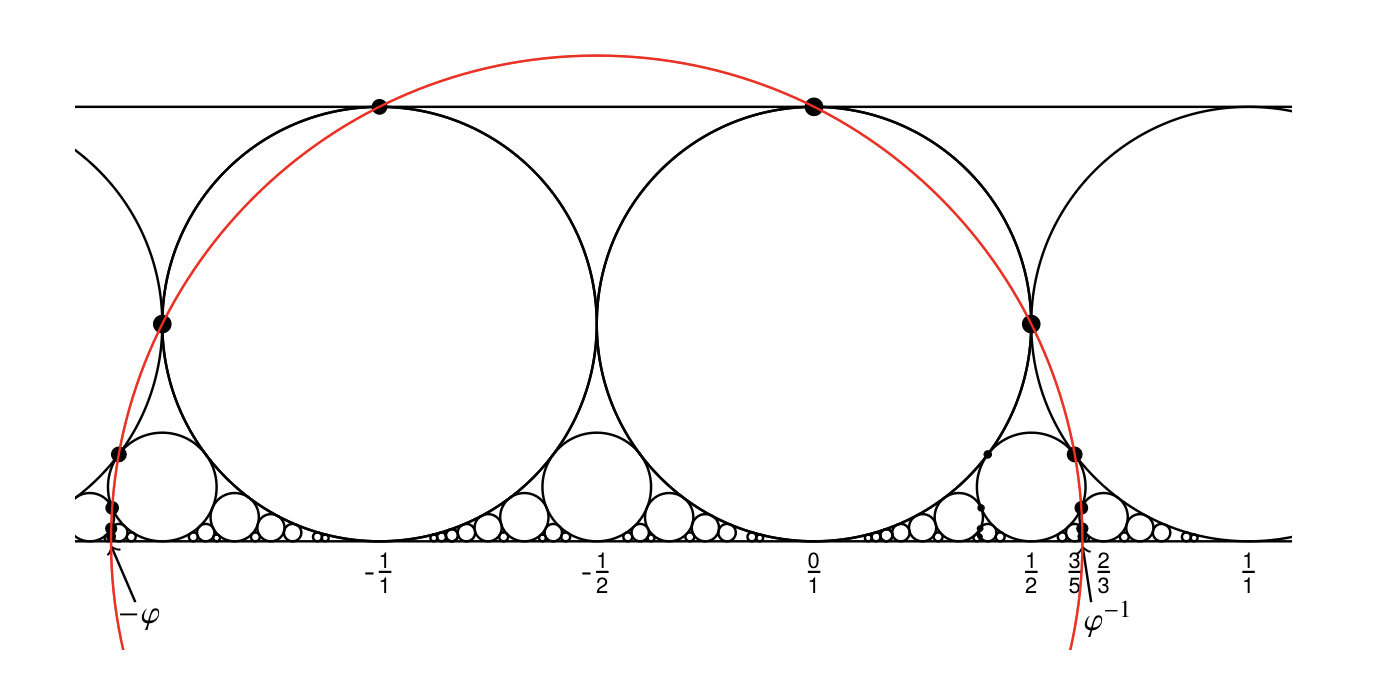
\includegraphics[width=0.5\linewidth]{截屏2024-03-30 下午6.03.37.png}
        \caption{Ford Circles[1]}
        \label{fig:enter-label}
    \end{figure}


 

  \end{block}
\end{column}{\colwidth}
\separatorcolumn

\begin{column}{\colwidth}
\newline
\newline
\newline
\textbf{Definition:} Let $K[p,m]$ be a circle of radius $\frac{1}{2m^2}$ tangent to x-axis at $(\frac{p}{m},0)$.
 \newline
We are able to prove that the sequence of points are among points of tangency of a series of Ford circles $K[F_{n},F_{n+1}]$.
\newline

To prove this, we need two proposition of Ford circles.
\newline \textbf{Proposition 1:} two Ford circles $K[p,m]$ and $K[q,n]$ are tangent if  $det\begin{bmatrix}
    p & q \\
    m & n
\end{bmatrix} = \pm 1$ (We can prove this by using the fact that the distance between the center of two tangent circles are exactly the sum of their radius).
\newline 

\textbf{Proposition 2:} The point of tangency of two tangent Ford circles is $(\frac{pm+qn}{m^2+n^2}, \frac{1}{m^2 + n^2})$ (We can prove this using the fact that $(\frac{q}{n} - x):(x - \frac{p}{m}) = R:r$ ).

\begin{figure}
    \centering
    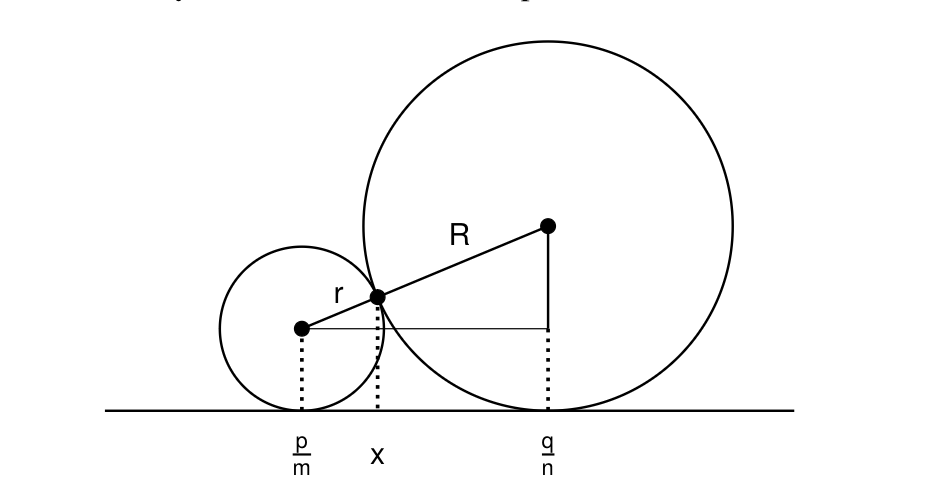
\includegraphics[width=0.5\linewidth]{截屏2024-03-30 下午6.31.26.png}
    \caption{Proposition 2[1]}
    \label{fig:enter-label}
\end{figure}
We first prove that the series of Ford circles are tangent to each other. This can be simply proved by the fact that 

    $$det\begin{bmatrix}
    F_{n-1} & F_{n} \\
    F_{n} & F_{n+1}
\end{bmatrix} = (-1)^n$$
  
  
  Then we prove that the point of tangency is exactly $(\frac{F_{2n}}{F_{2n+1}},\frac{1}{F_{2n+1}})$.    This is because by proposition two point of tangency is $(\frac{F_{n-1}F_{n}+F_{n}F{n+1}}{F_{n}^2+F_{n+1}^2},\frac{1}{F_{n}^2+F_{n+1}^2})$  which is the same as $(\frac{F_{2n}}{F_{2n+1}},\frac{1}{F_{2n+1}})$ by Lemma 1.
  \begin{block}{Conclusion}
This poster obtained some important facts regarding the Fibonacci sequence. We showed that the golden ratio can be derived from the limit ratio of the Fibonacci sequence. We extended the Fibonacci sequence to two-dimension and found out that these points are on the same circles with a radius of the golden ratio. In addition, this poster connected the concept of Ford circles with the "two dimension Fibonacci sequence" and showed that all the points are among the points of tangency of a series of Ford circles. 
    



  \end{block}

  \begin{block}{References}

    \nocite{*}
    \footnotesize{[1]Kocik, Jerzy. (2020). Fibonacci numbers and Ford circles. }
    
    \footnotesize{[2]Clancy, T. (2008). The Fibonacci Numbers. \textit{Senior Project Archive, Whitman College}.. }

  \end{block}

\end{column}

\separatorcolumn
\end{columns}
\end{frame}

\end{document}
